\documentclass{article}
\usepackage{setspace}
\usepackage{listings}
\usepackage{color}
\usepackage{amsmath}
\usepackage{amssymb}
\usepackage{amsthm}
\usepackage{graphicx} 
\usepackage{float} 
\usepackage{fancyhdr}                                
\usepackage{lastpage}                                           
\usepackage{layout}   
\usepackage{subfigure} 
\definecolor{codegreen}{rgb}{0,0.6,0}
\definecolor{codegray}{rgb}{0.5,0.5,0.5}
\definecolor{codepurple}{rgb}{0.58,0,0.82}
\definecolor{backcolour}{rgb}{0.95,0.95,0.92}

\lstdefinestyle{mystyle}{
    backgroundcolor=\color{backcolour},   
    commentstyle=\color{codegreen},
    keywordstyle=\color{magenta},
    numberstyle=\tiny\color{codegray},
    stringstyle=\color{codepurple},
    basicstyle=\footnotesize,
    breakatwhitespace=false,         
    breaklines=true,                 
    captionpos=b,                    
    keepspaces=true,                 
    numbers=left,                    
    numbersep=5pt,                  
    showspaces=false,                
    showstringspaces=false,
    showtabs=false,                  
    tabsize=2
}
\pagestyle{fancy}  
\lhead{ZHANG HUAKANG}
\chead{Assignment 2} 
\rhead{DB92760} 
\renewcommand{\baselinestretch}{1.05}
\title{Assignment 2 of CISC 2002}
\author{ZHANG Huakang/DB92760}

\begin{document}
    \maketitle
    \section{}
        \lstinputlisting[language=Matlab,style=mystyle,caption=Function]{code/Assignment_2_1_f.m}
        \lstinputlisting[language=Matlab,style=mystyle,caption=Derivative]{code/Assignment_2_1_derivative.m}
        \subsection{}
            \lstinputlisting[language=Matlab,style=mystyle,caption=Bisection]{code/Assignment_2_1_1.m}
            \lstinputlisting[style=mystyle,caption=Bisection Output]{code/Assignment_2_1_1_output}
        \subsection{}
            \lstinputlisting[language=Matlab,style=mystyle,caption=Newton's Method]{code/Assignment_2_1_2.m}
            \lstinputlisting[style=mystyle,caption=Newton's Method Output]{code/Assignment_2_1_2_output}

    \section{}
        \lstinputlisting[language=Matlab,style=mystyle,caption=Function]{code/Assignment_2_2_f.m}
        \lstinputlisting[language=Matlab,style=mystyle,caption=Matlab Code]{code/Assignment_2_2.m}
        \lstinputlisting[style=mystyle,caption=Output]{code/Assignment_2_2_output}
    \section{}
        
            \paragraph{
            When $\epsilon_n=\frac{1}{10^n}$
                \begin{equation*}
                    \begin{split}
                        \epsilon_n=&\frac{1}{10^n}\\
                            =&\frac{1}{10}\epsilon_{n-1}\\
                        r-\epsilon_n=&r-\frac{1}{10}\epsilon_{n-1}\\
                            =&r-\epsilon_{n-1}+\frac{9}{10}\epsilon_{n-1}\\
                        \frac{r-\epsilon_n}{r-\epsilon_{n-1}}=&1+\frac{\frac{9}{10}\epsilon_{n-1}}{r-\epsilon_{n-1}}\\
                            =&1+\frac{\frac{9}{10}\epsilon_{n-1}}{0-\epsilon_{n-1}}\\
                            =&1-\frac{9}{10}\\
                            =&\frac{1}{10}\\
                        \lim_{n\rightarrow \infty} |\frac{r-\epsilon_n}{r-\epsilon_{n-1}}|=&\lim_{n\rightarrow \infty}| \frac{1}{10}|\\
                            =&\frac{1}{10}
                    \end{split}
                \end{equation*}
                Therefore, the rate of convergence $\mu=\frac{1}{10}$, and the order of convergence $p=1$
            }
                \paragraph{
            When $\epsilon_n=\frac{1}{100^n}$
            \begin{equation*}
                \begin{split}
                    \epsilon_n=&\frac{1}{100^n}\\
                        =&\frac{1}{100}\epsilon_{n-1}\\
                    r-\epsilon_n=&r-\epsilon_{n-1}+\frac{99}{100}\epsilon_{n-1}\\
                    \frac{r-\epsilon_n}{r-\epsilon_{n-1}}=&1+\frac{\frac{99}{100}\epsilon_{n-1}}{r-\epsilon_{n-1}}\\
                        =&1-\frac{99}{100}\\
                        =&\frac{1}{100}\\
                    \lim_{n\rightarrow \infty} |\frac{r-\epsilon_n}{r-\epsilon_{n-1}}|=&\lim_{n\rightarrow \infty}|\frac{1}{100}|\\
                        =&\frac{1}{100}\\
                \end{split}
            \end{equation*}
            Therefore, the rate of convergence $\mu=\frac{1}{100}$, and the order of convergence $p=1$
                }
                \paragraph{
                    When $\epsilon_n=\frac{1}{2^{w^n}}$
                    \begin{equation*}
                        \begin{split}
                            \epsilon_n=&\frac{1}{2^{2^n}}\\
                                =&(\frac{1}{2^{2^{n-1}}})^2\\
                                =&\epsilon_{n-1}^2\\
                            r-\epsilon_n=&r-{\epsilon_{n-1}}^2\\
                            \frac{r-\epsilon_n}{r-\epsilon_{n-1}}=&\frac{r-\epsilon_{n-1}^2}{r-\epsilon_{n-1}}\\
                                =&\frac{-\epsilon_{n-1}^2}{-\epsilon_{n-1}}\\
                                =&\epsilon_{n-1}\\
                            \lim_{n\rightarrow\infty} |\frac{r-\epsilon_n}{r-\epsilon_{n-1}}|=&\lim_{n\rightarrow\infty}|\epsilon_{n-1}|\\
                                =&0
                        \end{split}
                    \end{equation*}
                    Therefore, the rate of convergence $\mu=0$, and the order of convergence $p=1$
                }


                \subsection*{}
                \lstinputlisting[language=Matlab,style=mystyle,caption=Matlab Code]{code/Assignment_2_3.m}
            \begin{figure}[H] 
                \centering 
                    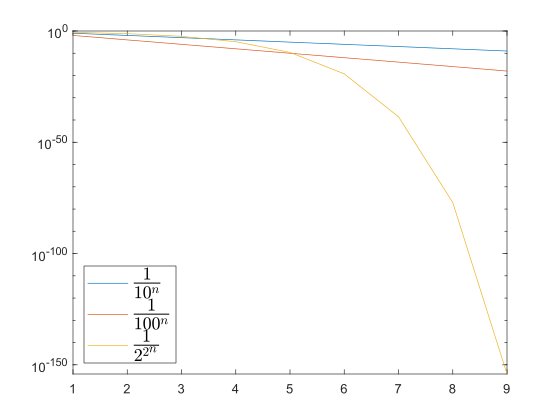
\includegraphics[width=0.9\textwidth]{img/Assignement_2_3.jpg}
                    \caption{Output} 
            \end{figure}
   
\end{document}